\chapter{Introduction}\label{chap:intro}

Wearable Cognitive Assistance (WCA) applications provide guidance to users for
a specific task.
This task could range from assembling a physical object, remembering people's
names, exercising, or playing a game or sport.
These applications
utilize mobile devices, such as smart glasses or a smartphone, to capture data
and interact with the user.
WCA applications process captured data in order to determine the physical state
of the task, and then provide assistance based on this physical state.

\hl{
  Table~{\ref{table:existing_wca}} lists some examples of WCA applications that
  have been developed prior to the work in this dissertation.}
All of these applications determine a task's physical state based on images from
an RGB camera.
This camera may be mounted on glasses that the user wears, or held in a tripod
with a view of the user's workspace.
Feedback is provided in the form of synthesized speech and images shown on the
display of the mobile device.

WCA is a compelling use case for edge computing. Many of these applications
utilize large deep neural network (DNN) models that are too computationally
intensive to run on a small and lightweight mobile device. However, these
applications generate large volumes of data that must be processed quickly.
Therefore, computation must be offloaded to a server with close network
proximity to the mobile device that is capturing the data~\cite{satya14}. We
will henceforth refer to this server as a cloudlet.

This work focuses on WCA applications that help users complete physical
assembly tasks.
Users are given step by step instructions, which requires the application to
determine when a user has completed a step of the task.
The application accomplishes this by processing frames from an RGB camera.
\hl{Prior to the work reported here, applications had been
developed for a lego kit~{\cite{lego}}, a lamp~{\cite{lamp}}, and a toy
sandwich~{\cite{sandwich}}}.
These tasks all required fewer than ten steps and
used parts that had distinct shapes and colors.
Taking WCA applications to the next level will require supporting tasks with
many more parts, many more steps, parts that are small relative to the full
object being assembled, and a combinatorial explosion of error states.
\hl{We address these challenges in this research.}

One significant challenge is the amount of labeled data that is required for
training computer vision models. Each
step of the task, and every error state that the developer would like to detect,
must be represented in the data that the models get trained on.
Increasing the number of steps thus directly increases the amount of data that
is required for training the models.
Collecting and labeling all of this data is an incredibly time-consuming
process.
This process can take up to 2 or 3 hours per task step.
\hl{Developing these models is an iterative process, which involves testing under
different lighting conditions, and then collecting more data in environments
in which the model performs poorly.}
Creating training sets is thus a significant barrier to developing WCA
applications that support large numbers of steps and large numbers of parts.

Assembly tasks might involve parts that are much smaller than the full object
being assembled.
For example, one step might require the user to insert a screw into a large
metal piece.
The application needs to be able to detect when steps involving small screws
have been completed, as well as steps involving larger parts.
In addition, there are many possible ways that a user can complete a task step
incorrectly.
In fact, the number of possible errors that a person can make while completing a
task is significantly larger than the number of steps that are required to
complete the task.
\hl{These challenges lead to my thesis statement}.

\section{Thesis Statement}

\textbf{
  Scaling up WCA to complex assembly tasks is challenging because of
  (a) the difficulty of
  vision-based state detection with very small parts in the context of much
  larger objects being assembled; (b) the combinatorial explosion
  of possible error states; and (c) the large manual effort needed to create
  accurate DNNs that can reliably determine when task steps have been completed.
  These problems can be solved by a combination of (1) hierarchical
  decomposition of
  complex assemblies into modular compositions of subassemblies, (2) on-demand
  seamless
  escalation for live expert assistance, and (3) synthetic generation of
  training
  sets for born-digital components. The resulting solution can be implemented in
  a scalable and maintainable way using modular software components.
  This will enable the development of WCA applications for more complex tasks,
  which is a necessary step along the path towards making WCA applications
  practical for real world tasks.
}

\section{Potential Impact}

The following issues currently make WCA applications impractical for real world
assembly tasks:
\begin{itemize}
\item \hl{Current techniques do not support tasks with more than ten steps, and the
    steps must have gross visible differences from each other.
    For example, a WCA application developed with these techniques cannot detect
  the presence or absence of a single screw.
  Figure~{\ref{fig:subtle_gross}} shows an example of the gross differences that
  current techniques support, and the subtle differences that require the
  techniques introduced in this work.}
\item A developer must collect and label training data for each error state
  that the application detects.
  However, there are exponentially more error states than correct
  states for any given task.
  \hl{This makes it infeasible to create a WCA application that is capable of
  detecting all possible error states for a task.}
\item The computer vision models that we use for WCA applications require
  thousands of images depicting each state.
  All of these images must be labeled with a bounding box.
  Collecting and labeling these images requires an immense manual effort.
\end{itemize}

This thesis addresses all three of these issues.
We present new techniques that enable the development of WCA apps with steps
that look almost identical.
The changes between these steps are subtle, such as the addition of a single
screw.
Our techniques also enable the development of tasks with a larger number of
steps.

\begin{figure}
  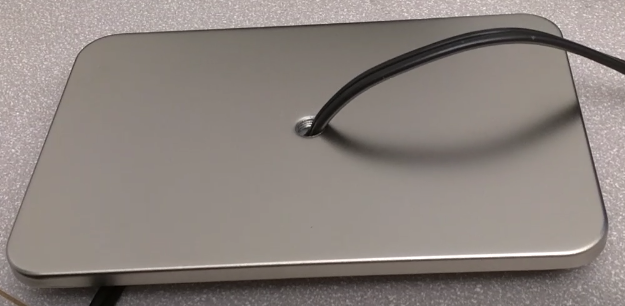
\includegraphics[width=0.5\textwidth]{figures/coarse_fine/lamp_base.png}
  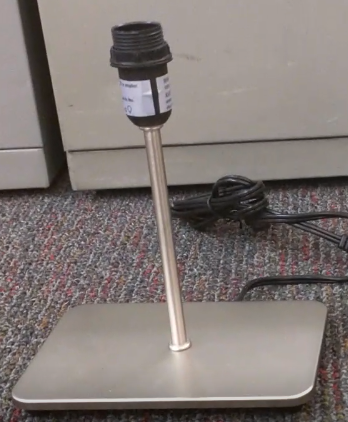
\includegraphics[width=0.5\textwidth]{figures/coarse_fine/lamp_pipe.png}
  
\includegraphics[width=0.5\textwidth]{figures/coarse_fine/stirling_1screw.png}
  
\includegraphics[width=0.5\textwidth]{figures/coarse_fine/stirling_2screws.png}
  \caption{
    The top two images illustrate a gross difference that current WCA techniques
    can detect.
    The bottom two images show a subtle difference that requires the new
    techniques from this work to support.
  }\label{fig:subtle_gross}
\end{figure}

Existing WCA applications for assembly tasks have no way of handling user
errors that they were not specifically developed to support.
If a user makes such a mistake, the application will either provide
the user with an instruction for a different step, that it was built to
recognize, or it might not provide any guidance at all.
\hl{In these cases, we allow the user to start a video call with a human who is
  an expert on the task that the user is trying to complete.
  We call this feature human escalation.
}

Lastly, reducing the time it takes for developers to build WCA applications for
assembly tasks is imperative for motivating a critical mass of developers to
build them.
\hl{
  Training computer vision models using synthetic data entirely removes the need
  to manually capture
  images of each task step and label these images with bounding boxes.
}

\section{Novelty}

\hl{
  Existing WCA applications used techniques that cannot support assembly tasks
  with large numbers of steps or subtle differences between steps.
  An example of a subtle difference is the insertion or removal of a single
  screw (as depicted in Figure~{\ref{fig:subtle_gross}}).
}
The lego application developed by \citet{chen2017} guided users to place colored
blocks on a 3D grid.
This application did not use any machine learning (ML) models, and its
techniques are tightly coupled to this specific task.
The Sandwich application developed by \citet{chen2017} determined the task step
that was shown using a single Faster R-CNN object detector.
As we describe in \S\ref{sec:single_model}, a single Faster R-CNN object
detector is not sufficient for more realistic tasks.

The combinatorial explosion of possible error states has not been addressed in
any prior work on WCA applications.
The sandwich application from \citet{chen2017} was built to detect one specific
error.
But none of our prior work has attempted to address the wide range of possible
mistakes that a well-intentioned user might make when completing an assembly
task.
Escalation to a human expert is the first solution that has been proposed.

Training ML models using synthetic images has long been an area of active
research.
However, this thesis represents the first attempt to do so in the context of
WCA.
We offer results from training models for real WCA applications, using synthetic
data.

\section{Roadmap}

This dissertation validates the thesis as follows:
\begin{itemize}
\item Chapter~\ref{chap:background} discusses prior work on WCA, other work on
  aids for assembly tasks, and the computer vision research that we leverage in
  our work.
\item Chapter~\ref{chap:detection} describes how we detect when steps of real
  world tasks have been completed.
  It also presents the three WCA applications that we developed using our
  techniques.
\item Chapter~\ref{chap:synthetic} presents and evaluates our efforts to train
  DNNs for WCA applications using synthetic training images.
\item Chapter~\ref{chap:escalation} introduces our system for error handling
  with human task experts.
  The chapter also presents Monte Carlo simulations that call center operators
  can use to determine the number of human experts that are required to support
  a set of WCA application users.
\item Chapter~\ref{chap:implementation} describes the software framework that
  we built to support Gabriel applications, and it explores how mobile device
  hardware can be used by WCA applications.
\item Chapter~\ref{chap:conclusion} concludes the dissertation and offers
  suggestions for future work on WCA applications.
\end{itemize}
